\documentclass[conference]{IEEEtran}

\usepackage{cite}
\usepackage{amsmath}
\usepackage{amssymb}
\usepackage{graphicx}
\usepackage{booktabs}
\usepackage{multirow}
\usepackage{url}
\usepackage{float}
\usepackage[hidelinks]{hyperref}

\graphicspath{{../results/plots/}{.}}

\title{Portfolio-Aligned PatchTST with Dynamic Relational Graphs for Cross-Sectional Return Forecasting in the NIFTY 100}

\author{
\parbox{0.98\textwidth}{\centering
\begin{tabular}{@{}c@{\hspace{0.01\textwidth}}c@{}}
\parbox[t]{0.47\textwidth}{\centering
Karthik Prabhu\\
Department of Computer Science and Engineering\\
PES University, Bengaluru, India\\
karthikprabhu711@gmail.com}
&
\parbox[t]{0.47\textwidth}{\centering
Arulmozhi Varma\\
Department of Computer Science and Engineering\\
PES University, Bengaluru, India\\
arul.ks2004@gmail.com}
\end{tabular}
\\[1.3em]
\begin{tabular}{@{}c@{\hspace{0.01\textwidth}}c@{}}
\parbox[t]{0.47\textwidth}{\centering
Karthik S Jasti\\
Department of Computer Science and Engineering\\
PES University, Bengaluru, India\\
karthikchess2005@gmail.com}
&
\parbox[t]{0.47\textwidth}{\centering
Dr. Ashwini M. Joshi\\
Associate Professor\\
Department of Computer Science and Engineering\\
PES University, Bengaluru, India\\
ashwinimjoshi@pes.edu}
\end{tabular}
}
}

\begin{document}
\maketitle

\begin{abstract}
This paper presents a portfolio-aligned deep learning framework for cross-sectional return forecasting in the NIFTY 100 universe. The objective is not to predict raw stock prices, but to rank stocks by expected forward performance and evaluate the ranking through a transaction-cost-aware long--short portfolio. Each stock is represented by a 128-trading-day window of engineered OHLCV, momentum, volatility, volume, market-relative, and sector-relative features. A three-branch multi-scale PatchTST encoder extracts temporal representations from patch lengths of 8, 16, and 32 days. These stock embeddings are then refined with a multi-relational graph attention module built from sector membership, rolling return correlation, and embedding similarity. The final representation is concatenated with market-regime features and optimized through three supervised heads: 5-day residual-return regression, cross-sectional ranking, and ternary direction classification. The system is evaluated using a walk-forward protocol over 2015--2024 with 5-year training, 1-year validation, and 1-year test windows rolled every six months. The configured saved run achieves an information coefficient (IC) of 0.0189, Rank IC of 0.0140, 57.90\% annualized return, and Sharpe ratio of 1.49 after 10 basis points transaction cost. A fixed-score robustness sweep on the same predictions shows that direct ranking-head execution reaches 90.93\% annualized return and a Sharpe ratio of 2.05. Baseline and ablation experiments show that pretraining, regime conditioning, and graph-based relational reasoning are important, while also showing that a strong tabular MLP is competitive with the configured execution score. The findings support PatchTST-plus-graph modeling as a useful research framework for Indian large-cap stock selection, but the observed drawdown near 65\% indicates that additional portfolio risk control is required before practical deployment.
\end{abstract}

\begin{IEEEkeywords}
Stock return forecasting, PatchTST, graph attention networks, cross-sectional ranking, portfolio construction, NIFTY 100, walk-forward evaluation
\end{IEEEkeywords}

\section{Introduction}
Cross-sectional stock forecasting is a difficult prediction problem because the signal-to-noise ratio of short-horizon returns is low, market regimes change over time, and each stock's behavior is influenced by sector, index, liquidity, and peer effects. A forecasting model that performs well on a pointwise error metric may still fail as an investment model if its ranking is unstable, if turnover is too high, or if performance disappears after transaction costs. For this reason, the present work treats stock prediction as a portfolio-aligned ranking problem rather than as a raw price-forecasting task.

Traditional portfolio theory connects security selection with risk-adjusted portfolio outcomes \cite{markowitz1952portfolio,sharpe1966mutual}. Modern machine learning extends this idea by learning nonlinear predictors from historical features, but financial evaluation must still respect chronological splits, transaction costs, and changing market regimes. Random train--test splits are inappropriate for this setting because they leak future regime information into training. This paper therefore uses a walk-forward design, a common practical requirement in financial machine learning \cite{lopezdeprado2018advances}.

Recent stock prediction work has moved from independent single-asset models toward architectures that jointly model temporal patterns and inter-stock relations. Temporal Relational Ranking (RSR) introduced relation-aware ranking for stocks \cite{feng2019temporal}. MASTER later showed that transformer-based market-guided stock encoders can improve cross-sectional signal quality \cite{li2024master}. In parallel, PatchTST demonstrated that patching long time series into tokens can improve transformer efficiency and representation quality \cite{nie2023patchtst}. These ideas motivate the central design of this project: encode each stock's temporal history with a multi-scale PatchTST backbone, then refine the stock embeddings through relational graph attention before portfolio evaluation.

The main contributions are as follows:
\begin{enumerate}
    \item an end-to-end NIFTY 100 cross-sectional forecasting pipeline that combines engineered financial features, multi-scale PatchTST, dynamic relational graphs, market-regime conditioning, and multi-task learning;
    \item a reviewer-transparent implementation and evaluation protocol using walk-forward testing, overlap-safe aggregation, transaction costs, significance testing, baseline comparison, ablation analysis, and robustness checks;
    \item empirical evidence that the architecture extracts positive out-of-sample cross-sectional signal in Indian large-cap equities, while also identifying important limitations such as high drawdown and strong competition from a tabular MLP baseline.
\end{enumerate}

\section{Literature Review / Related Work}
Early financial forecasting models focused on linear dependence and volatility clustering. ARCH and GARCH models established that conditional volatility is time-varying and predictable to some degree \cite{engle1982autoregressive,bollerslev1986generalized}. These models remain important for risk modeling, but they are not designed to learn nonlinear cross-sectional rankings from many stock-level features.

Machine learning methods broadened the forecasting toolkit. Krauss \emph{et al.} compared deep neural networks, random forests, and gradient-boosted trees for statistical arbitrage on S\&P 500 stocks \cite{krauss2017deep}. Fischer and Krauss showed that LSTM networks can improve directional stock prediction compared with simpler benchmarks \cite{fischer2018deep}. Gu \emph{et al.} demonstrated that machine learning methods can explain and predict asset returns using a large panel of firm characteristics \cite{gu2020empirical}. These studies support the use of nonlinear models, but many such systems treat stocks independently or focus on tabular features.

Sequence models and transformers address temporal structure more directly. The transformer architecture introduced attention-based sequence modeling \cite{vaswani2017attention}; Temporal Fusion Transformers adapted attention to interpretable multi-horizon forecasting \cite{lim2021temporal}; and PatchTST showed that patch tokens can be effective for long-horizon time-series forecasting \cite{nie2023patchtst}. For stock selection specifically, relation-aware models are especially relevant. RSR models temporal stock relations for ranking \cite{feng2019temporal}, MASTER combines market-guided feature selection with transformer-style stock modeling \cite{li2024master}, and graph attention methods provide a natural mechanism for learning relation-specific neighbor influence \cite{velickovic2018gat,kipf2017semi}.

Learning-to-rank and graph-based portfolio studies are closest to the present work. Zhang \emph{et al.} formulated long--short stock construction as a listwise ranking problem \cite{zhang2022listwise}. Gorduza \emph{et al.} used analyst-network graph attention to extract alpha from relational structure \cite{gorduza2024analyst}. The present work follows the same broad view that portfolio value depends more on cross-sectional ranking quality than on isolated point forecasts, but applies it to the Indian NIFTY 100 universe with a PatchTST-plus-multi-relational-graph architecture.

\begin{table*}[t]
\centering
\caption{Summary of ten representative related studies and their relevance to this work.}
\label{tab:related_work}
\footnotesize
\setlength{\tabcolsep}{3pt}
\begin{tabular}{p{3.0cm}p{0.9cm}p{2.1cm}p{2.7cm}p{4.0cm}p{3.2cm}}
\toprule
Study & Year & Market / Domain & Main method & Main contribution & Relevance to this paper \\
\midrule
Engle \cite{engle1982autoregressive} & 1982 & Financial returns & ARCH & Modeled time-varying conditional volatility & Motivates volatility and regime features \\
Krauss \emph{et al.} \cite{krauss2017deep} & 2017 & S\&P 500 & DNN, random forest, gradient boosting & Showed machine learning value for statistical arbitrage & Motivates nonlinear baselines \\
Fischer and Krauss \cite{fischer2018deep} & 2018 & S\&P 500 & LSTM & Applied sequence deep learning to stock movement prediction & Motivates temporal encoders \\
Feng \emph{et al.} \cite{feng2019temporal} & 2019 & US equities & Temporal relational ranking & Introduced relation-aware stock ranking & Directly motivates ranking and relations \\
Gu \emph{et al.} \cite{gu2020empirical} & 2020 & US equities & Machine learning asset pricing & Demonstrated predictive value of nonlinear asset-pricing models & Supports cross-sectional ML framing \\
Lim \emph{et al.} \cite{lim2021temporal} & 2021 & Time-series forecasting & Temporal Fusion Transformer & Combined attention, covariates, and multi-horizon forecasting & Supports transformer-style time-series modeling \\
Zhang \emph{et al.} \cite{zhang2022listwise} & 2022 & China A-shares & Listwise learning-to-rank & Optimized stock ordering for long--short portfolios & Supports portfolio-ranking objective \\
Nie \emph{et al.} \cite{nie2023patchtst} & 2023 & General time series & PatchTST & Showed patch-token transformers are efficient for long sequences & Provides temporal backbone idea \\
Li \emph{et al.} \cite{li2024master} & 2024 & Chinese equities & Market-guided stock transformer & Improved IC and Rank IC with market-guided stock modeling & Closest transformer stock benchmark \\
Gorduza \emph{et al.} \cite{gorduza2024analyst} & 2024 & US equities & Analyst-network graph attention & Extracted alpha from structured stock relations & Supports graph-based relational alpha \\
\bottomrule
\end{tabular}
\end{table*}

\section{Proposed Architecture / Methodology}
\subsection{Problem Definition}
Let $i \in \{1,\ldots,N\}$ denote a stock and $t$ denote a trading date. For each stock-date pair, the model observes a lookback tensor $X_{i,t} \in \mathbb{R}^{L \times F}$, where $L=128$ trading days and $F=27$ engineered stock features. The primary prediction target is the 5-day forward residual log return:
\begin{equation}
y^{\text{res}}_{i,t}=\log\left(\frac{P_{i,t+5}}{P_{i,t}}\right)-\log\left(\frac{M_{t+5}}{M_t}\right),
\end{equation}
where $P_{i,t}$ is the adjusted stock close and $M_t$ is the NIFTY 100 index level. Residualization removes broad index movement from the target so that the model focuses on stock-specific relative performance. The same 5-day horizon is also used to construct a ternary direction label through date-wise cross-sectional quantiles: bottom 30\% as down, middle 40\% as flat, and top 30\% as up.

\subsection{Feature Engineering and Normalization}
The feature builder constructs 27 stock-level variables from daily OHLCV data. These include log return, overnight return, intraday return, high--low range, close--open spread, 5/10/20/60-day momentum, 20-day drawdown, 5/10/20-day realized volatility, ATR-style volatility, volatility z-score, log volume, volume change, volume surprise, market-relative return, sector-relative return, relative-strength percentile, 20/60-day moving-average distance, 14-day RSI, Bollinger-band distance, and 5-day rolling log-price slope. Features are winsorized and standardized cross-sectionally within each date. This normalization is important because the model ranks stocks against peers on the same trading day rather than forecasting each stock in isolation.

Market-regime features are computed from the NIFTY 100 index and India VIX: VIX level, VIX percentage change, VIX z-score, 5-day market return, 20-day market volatility, and market trend. The configuration expects an 8-dimensional regime vector; the model pads the six computed regime fields when needed. This detail is important for reproducibility because it explains why the configured dimension is larger than the directly computed regime feature count.

\subsection{Temporal Patch Encoder}
For each stock, the temporal encoder converts the 128-day feature window into patch tokens. Three PatchTST branches use patch lengths $\{8,16,32\}$ and strides $\{4,8,16\}$, allowing the model to capture short, medium, and longer local patterns. Each branch applies linear patch projection, positional embeddings, transformer encoder layers, attention pooling, and final-token extraction. The pooled and final-token vectors from all three branches are concatenated and projected into a 128-dimensional stock embedding. This design follows the PatchTST insight that long time series can be represented efficiently as patch sequences \cite{nie2023patchtst}, while retaining the transformer attention mechanism introduced by Vaswani \emph{et al.} \cite{vaswani2017attention}.

\subsection{Multi-Relational Graph Reasoning}
After temporal encoding, the system constructs a graph over stocks for each date. Three relation types are used:
\begin{enumerate}
    \item sector relation, which fully connects stocks in the same sector;
    \item rolling-correlation relation, which connects historically correlated stocks using recent return windows;
    \item embedding-similarity relation, which connects stocks whose current temporal embeddings are close in cosine similarity.
\end{enumerate}
The graph encoder applies separate graph-attention transformations per relation and fuses their outputs with residual stock embeddings. In simplified form,
\begin{equation}
\tilde{h}_{i,t}=\operatorname{GAT}(h_{i,t},\mathcal{N}_{i,t}), \qquad
h^{\text{graph}}_{i,t}=h_{i,t}+\tilde{h}_{i,t},
\end{equation}
where $h_{i,t}$ is the temporal embedding and $\mathcal{N}_{i,t}$ is the set of relation-specific neighbors. Graph attention is used because it can assign different importance weights to different neighbors instead of averaging all related stocks equally \cite{velickovic2018gat}.

\subsection{Prediction Heads and Loss Function}
The final stock representation concatenates the graph-refined embedding with the regime vector. It is passed to three heads: a residual-return regression head, a ranking head, and a three-class direction head. The supervised objective is
\begin{equation}
\mathcal{L}=\lambda_{reg}\mathcal{L}_{\text{Huber}}+\lambda_{rank}\mathcal{L}_{\text{rank}}+\lambda_{dir}\mathcal{L}_{\text{focal}},
\end{equation}
with $\lambda_{reg}=1.0$, $\lambda_{rank}=0.75$, and $\lambda_{dir}=0.02$ in the configured run. The Huber loss provides robustness to extreme return observations \cite{huber1964robust}; the ranking loss uses a pairwise logistic objective; and focal loss reduces the impact of easy direction-classification examples \cite{lin2017focal}. Supervised training also applies exponential recency weighting with a 252-trading-day half-life, so recent training dates receive higher weight within each fold.

\subsection{Portfolio Execution Rule}
The configured execution score is a validation-tuned blend of return, ranking, and direction components after date-wise z-scoring. The portfolio rule is fixed after score construction: each rebalance selects the top $k=10$ stocks as equal-weight longs and the bottom $k=10$ stocks as equal-weight shorts. Weekly rebalancing and 10 basis points transaction cost are used for the primary result. A separate robustness sweep evaluates fixed score columns, including direct execution of the ranking head. The paper reports the configured blended-score run as the primary outcome and treats the stronger ranking-head portfolio as a robustness result, not as a replacement for the configured result.

\begin{figure*}[t]
\centering
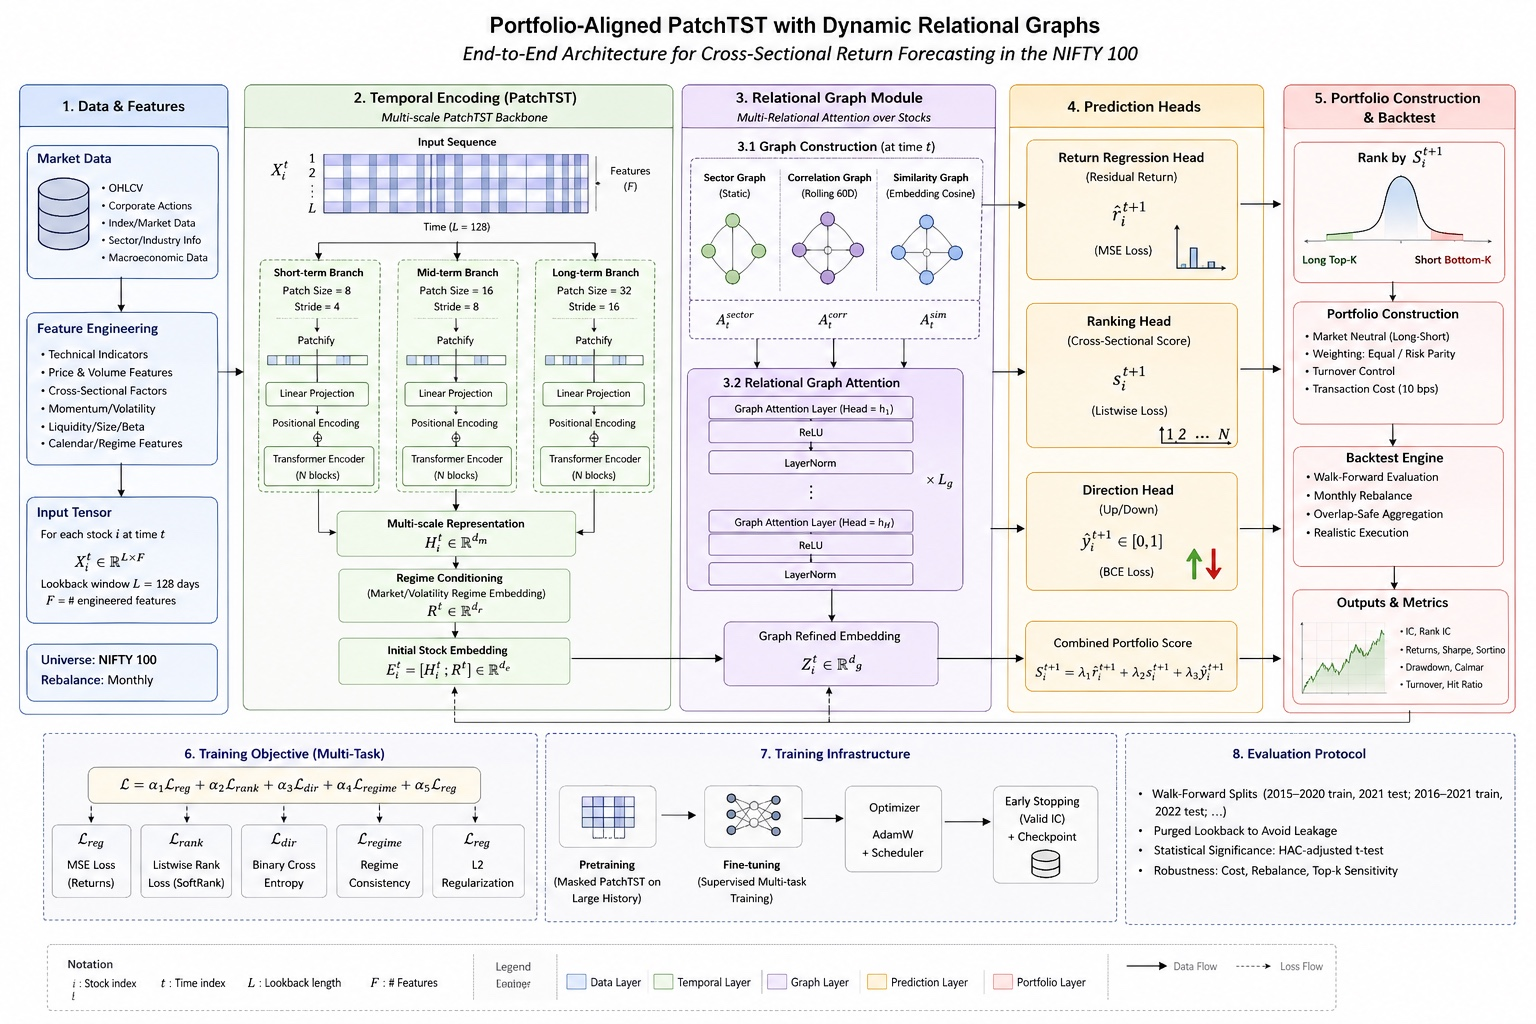
\includegraphics[width=\textwidth]{Final_Diagram.jpeg}
\caption{End-to-end architecture of the NIFTY 100 cross-sectional forecasting system. The pipeline downloads market data, builds stock and regime features, applies cross-sectional normalization, encodes each stock with multi-scale PatchTST, refines embeddings with multi-relational graph attention, predicts return/rank/direction outputs, and evaluates a transaction-cost-aware long--short portfolio.}
\label{fig:architecture}
\end{figure*}

\section{Implementation}
\subsection{Data Source and Universe}
The implementation uses daily Yahoo Finance data downloaded through the project scripts. Stock-level OHLCV data are combined with the NIFTY 100 index and India VIX. The configured study period is 2015-01-01 to 2024-12-31. The tracked universe file contains 99 ticker rows, while the saved experiments report an effective 97-name universe because two Yahoo Finance symbols were unavailable during ingestion. This distinction is stated explicitly because reviewers should not assume that all 100 nominal NIFTY 100 names were present in every run.

The raw and processed data directories are intentionally excluded from version control. Reproduction therefore requires rerunning the download and feature-building scripts. This also means that the experiment is based on a static universe file rather than point-in-time historical index membership. The resulting survivorship-bias risk is a limitation of the present research prototype.

\subsection{Pipeline Scripts}
The repository is organized as an executable research pipeline. The standard run sequence is: data download, feature construction, self-supervised pretraining, walk-forward supervised training, and evaluation/plot generation. Additional scripts produce significance tests, robustness dashboards, baseline comparisons, and ablation studies. Intermediate artifacts include per-ticker feature files, regime features, sector maps, trained checkpoints, prediction outputs, metrics tables, and plots.

\subsection{Training Configuration}
The main model uses 128-dimensional embeddings, four transformer encoder layers per PatchTST branch, four attention heads, dropout of 0.15, two graph-attention layers, and AdamW optimization. Adam-style adaptive optimization and decoupled weight decay are standard choices for deep neural network training \cite{kingma2015adam,loshchilov2019decoupled}. The configuration specifies 30 pretraining epochs, 50 supervised epochs, mixed precision, gradient checkpointing, weight decay of $10^{-4}$, supervised learning rate of $10^{-4}$, and early stopping on score Rank IC. The paper reports the saved results produced by this repository state; if future reruns change the epoch counts or data availability, the numbers should be regenerated and restated.

\subsection{Walk-Forward Evaluation}
The walk-forward protocol uses 5 years for training, 1 year for validation, and 1 year for testing, rolling forward every six months. This yields seven test folds. Because neighboring test windows overlap, aggregate reporting uses a latest-fold policy to de-duplicate dates before computing final metrics. This prevents the same out-of-sample date from being counted multiple times in the headline result.

Evaluation metrics include daily IC, Rank IC, top--bottom spread, top-$k$ precision, annualized return, Sharpe ratio, Sortino ratio, maximum drawdown, hit ratio, annualized turnover, and Calmar ratio. Portfolio evaluation follows the risk-adjusted tradition of performance measurement \cite{sharpe1966mutual}. Statistical evidence is reported using heteroskedasticity-and-autocorrelation-consistent (HAC) tests and bootstrap confidence intervals \cite{neweywest1987simple,efron1993introduction}.

\subsection{Baselines and Ablations}
Three cheap baselines are implemented: ridge regression, histogram gradient boosting, and a tabular MLP. Ridge regression is a classical regularized linear method \cite{hoerl1970ridge}; gradient boosting is a strong nonlinear tree-based reference \cite{friedman2001greedy}. For these baselines, each stock-date is represented by a 204-dimensional tabular vector containing the latest features, rolling summary statistics over 5/20/60-day windows, regime variables, and recent-return summaries. The ablation suite removes pretraining, ranking loss, regime features, or the graph module. All baselines and ablations reuse the same walk-forward evaluation logic as the main model.

\section{Results \& Discussion}
\subsection{Main Out-of-Sample Performance}
Table~\ref{tab:main_results} summarizes the main saved run and the strongest fixed-score robustness result. The configured blended-score run achieves positive IC, positive Rank IC, 57.90\% annualized return, and Sharpe ratio of 1.49 after transaction cost. The daily IC is small in absolute value, but this is typical for cross-sectional equity forecasting; the economic relevance comes from repeated ranking across many stocks and dates. The robustness-best ranking-head execution is stronger on annualized return and Sharpe, but it is reported separately because it was selected in a post-run fixed-score sweep.

\begin{table}[t]
\centering
\caption{Main out-of-sample results. The configured run uses the saved blended execution score. The robustness result uses the fixed ranking-head score on the same saved predictions.}
\label{tab:main_results}
\footnotesize
\begin{tabular}{lrr}
\toprule
Metric & Configured run & Rank-head robustness \\
\midrule
IC mean & 0.0189 & 0.0189 \\
Rank IC mean & 0.0140 & 0.0140 \\
Score Rank IC mean & 0.0156 & 0.0140 \\
Top--bottom spread & 0.00236 & 0.00248 \\
Top-$10$ precision & 0.5094 & 0.5079 \\
Annualized return & 57.90\% & 90.93\% \\
Sharpe ratio & 1.49 & 2.05 \\
Sortino ratio & 2.62 & 3.75 \\
Maximum drawdown & -64.98\% & -65.27\% \\
Annualized turnover & 83.98 & 84.04 \\
Hit ratio & 52.12\% & 52.12\% \\
\bottomrule
\end{tabular}
\end{table}

Fold-level results are mixed. Four of seven folds are positive on Sharpe and score Rank IC. The best fold reaches Sharpe 4.34, while the weakest fold reaches Sharpe -1.91. This pattern suggests that the model captures a real but regime-sensitive signal. It should not be presented as a uniformly stable alpha engine.

\begin{figure}[t]
\centering
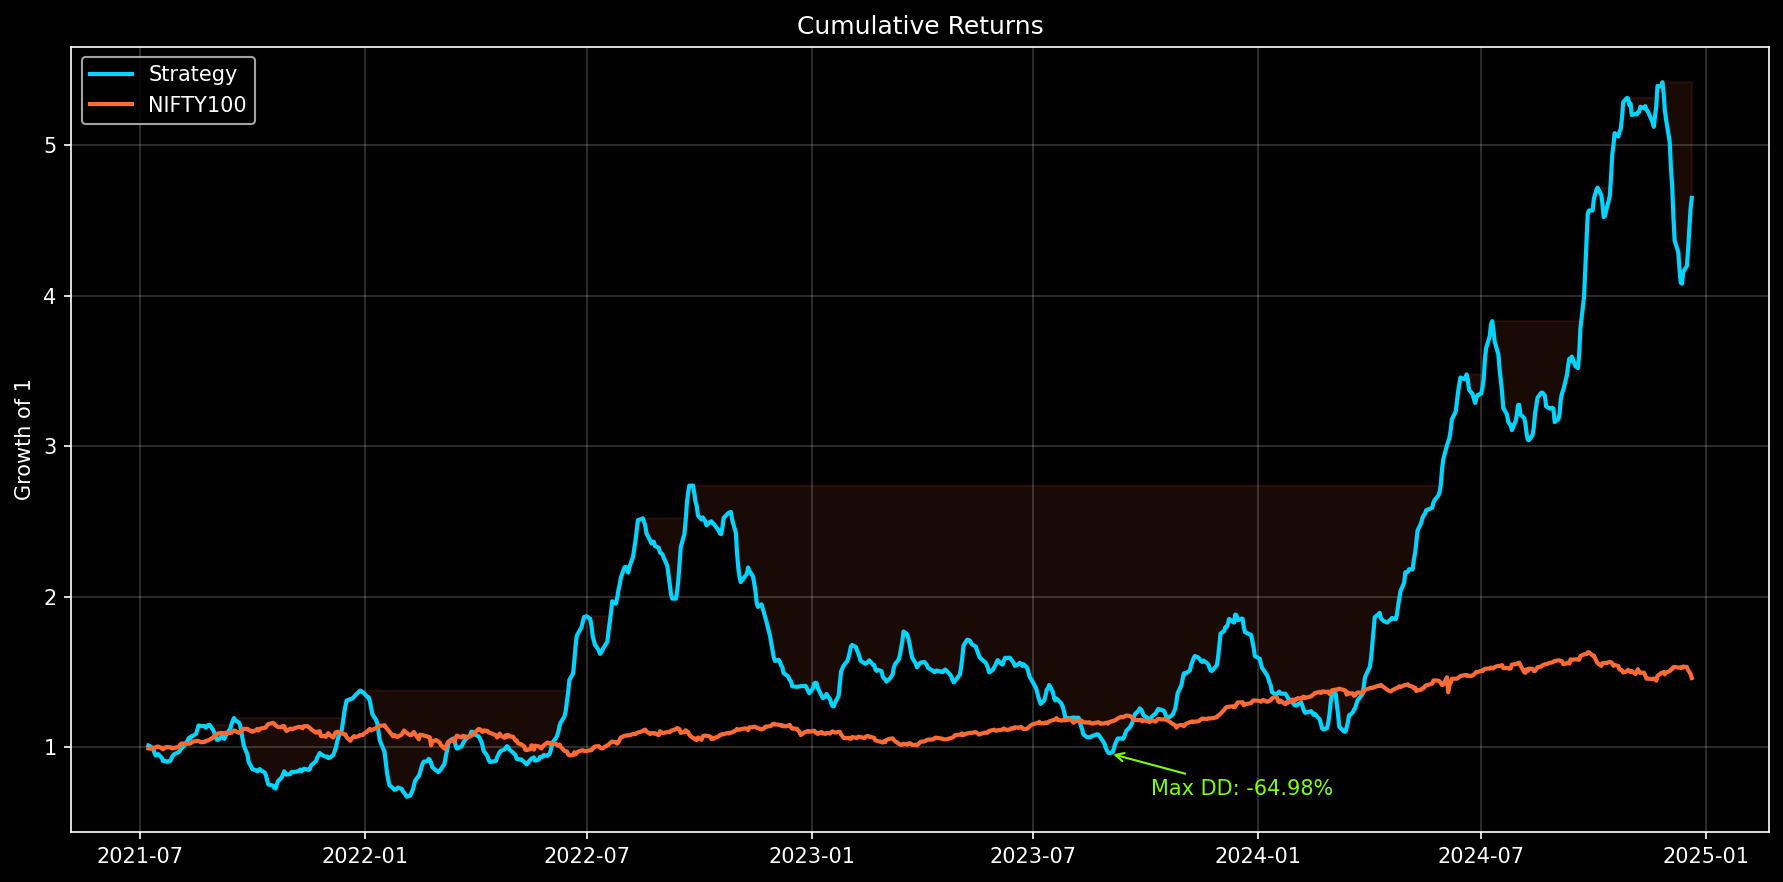
\includegraphics[width=\columnwidth]{portfolio_cumulative_returns.png}
\caption{Cumulative return of the configured portfolio compared with the NIFTY 100 benchmark series used by the evaluation script.}
\label{fig:portfolio_returns}
\end{figure}

\begin{figure}[t]
\centering
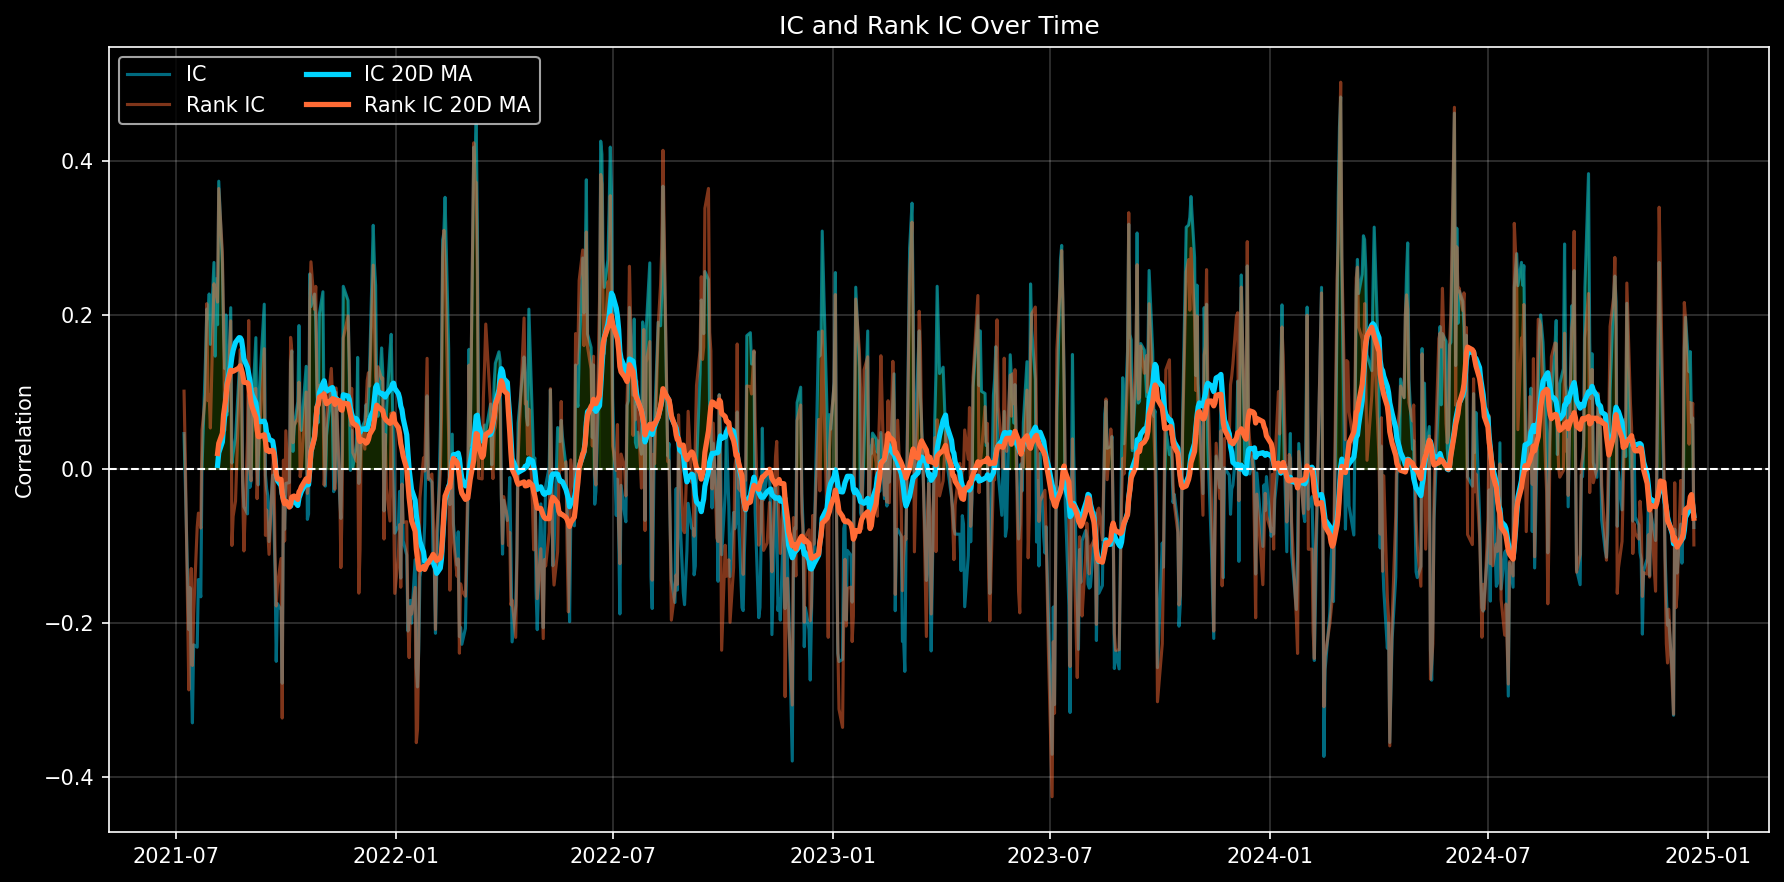
\includegraphics[width=\columnwidth]{ic_over_time.png}
\caption{Daily IC and Rank IC over the aggregated out-of-sample period. The rolling averages show that signal strength varies substantially across market regimes.}
\label{fig:ic_time}
\end{figure}

\subsection{Baseline Comparison}
Table~\ref{tab:baselines} compares the proposed model with the implemented baselines. The configured model clearly outperforms ridge regression and histogram gradient boosting on portfolio return and Sharpe. However, the tabular MLP is a strong competitor: it achieves higher IC, higher Rank IC, higher annualized return, higher Sharpe, and lower maximum drawdown than the configured blended-score model. This must be stated plainly to avoid overstating the contribution.

The correct interpretation is not that the temporal-relational architecture is useless. The ranking-head robustness result exceeds the MLP in annualized return and Sharpe, and the ablations show that graph structure, pretraining, and regime features materially affect behavior. The result instead shows that engineered tabular features already contain substantial predictive information and that execution-score design matters as much as neural architecture choice.

\begin{table*}[t]
\centering
\caption{Baseline comparison under the shared walk-forward evaluation protocol. Baselines are evaluated using their direct predicted return as the execution score.}
\label{tab:baselines}
\footnotesize
\begin{tabular}{llrrrrr}
\toprule
Method & Score used & IC & Rank IC & Ann. return & Sharpe & Max DD \\
\midrule
Ridge & predicted return & 0.0137 & 0.0078 & 6.78\% & 0.36 & -63.66\% \\
HistGradientBoosting & predicted return & 0.0282 & 0.0156 & -0.74\% & 0.15 & -67.32\% \\
MLP & predicted return & 0.0290 & 0.0225 & 60.05\% & 1.65 & -45.57\% \\
Proposed (configured) & alpha\_score & 0.0189 & 0.0140 & 57.90\% & 1.49 & -64.98\% \\
Proposed (rank-head robustness) & rank head & 0.0189 & 0.0140 & 90.93\% & 2.05 & -65.27\% \\
\bottomrule
\end{tabular}
\end{table*}

\subsection{Ablation Study}
Table~\ref{tab:ablations} reports the targeted ablations. Removing pretraining causes IC to become negative and annualized return to fall below zero. Removing regime features produces negative annualized return and the worst drawdown in the table, showing that market context is essential. The temporal-only model retains positive IC and Rank IC but loses portfolio value, implying that temporal features alone are not sufficient for this execution rule. Removing the ranking loss produces a positive portfolio result, but its ranking-head behavior becomes less aligned with the intended explicit ranking objective.

\begin{table}[!t]
\centering
\caption{Targeted ablation study. All variants use the same data pipeline, walk-forward folds, and evaluation logic as the configured full model.}
\label{tab:ablations}
\scriptsize
\setlength{\tabcolsep}{2.4pt}
\begin{tabular}{lrrrrrr}
\toprule
Variant & IC & RIC & Score RIC & Ann. Ret. & Sharpe & Max DD \\
\midrule
Full model & 0.0189 & 0.0140 & 0.0156 & 57.90\% & 1.49 & -64.98\% \\
No pretraining & -0.0026 & 0.0065 & 0.0014 & -3.88\% & 0.06 & -74.18\% \\
No regime & 0.0085 & 0.0069 & 0.0085 & -24.91\% & -0.56 & -81.43\% \\
Temporal only & 0.0190 & 0.0187 & 0.0191 & 0.67\% & 0.19 & -78.06\% \\
No ranking loss & 0.0220 & -0.0113 & 0.0201 & 65.88\% & 1.48 & -63.06\% \\
\bottomrule
\end{tabular}
\end{table}

\begin{figure}[t]
\centering
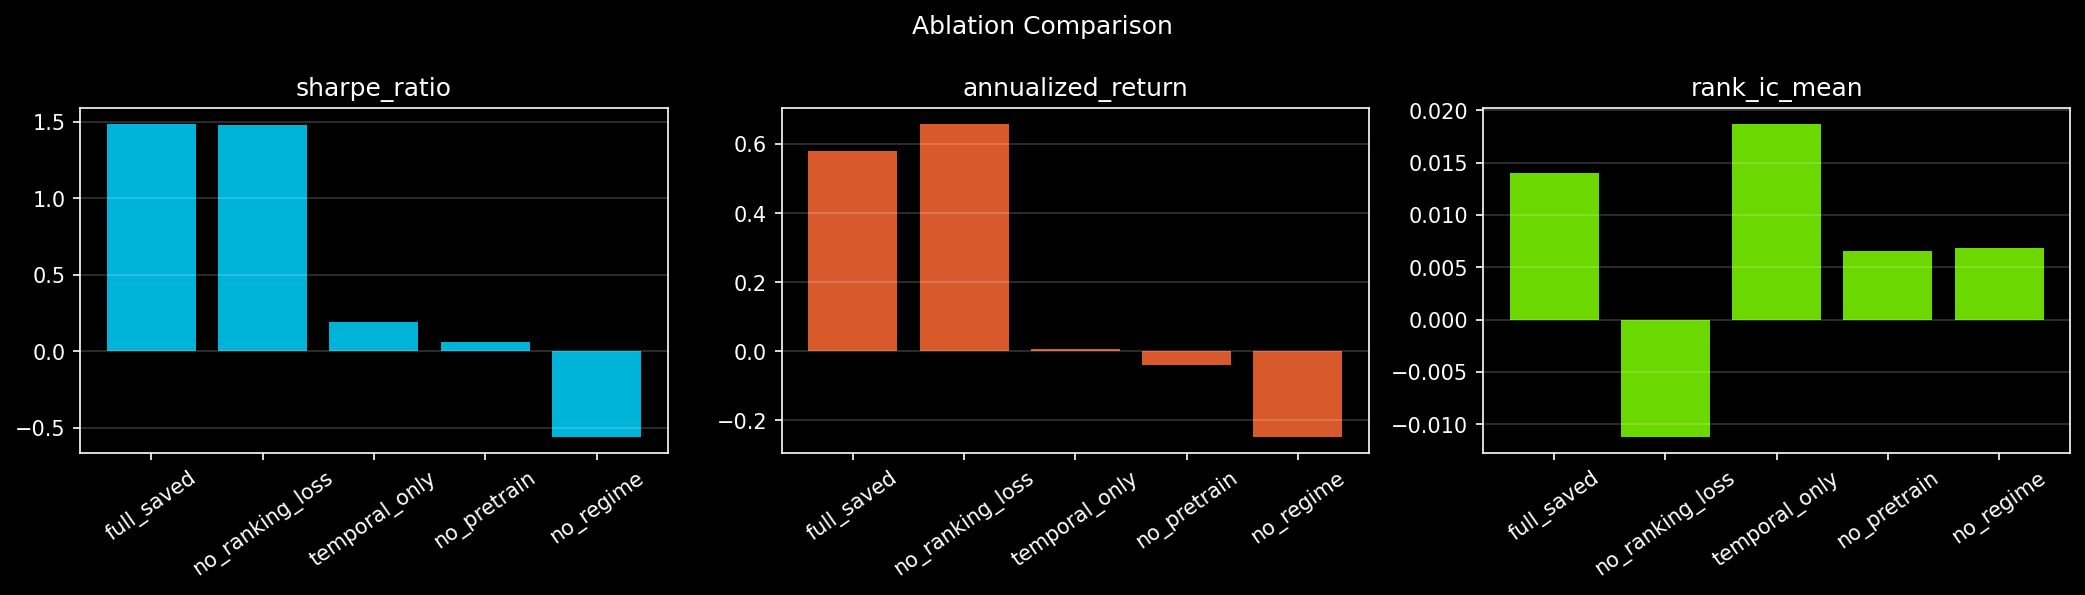
\includegraphics[width=\columnwidth]{ablations_comparison.png}
\caption{Ablation comparison generated from the saved metrics. The graph module, regime context, and pretraining materially change portfolio behavior.}
\label{fig:ablation_plot}
\end{figure}

\vspace{-1.2em}
\subsection{Significance and Robustness}
Table~\ref{tab:significance} reports statistical tests on daily metrics. IC is statistically positive at the 5\% level with HAC-adjusted $p=0.0437$. Rank IC, score Rank IC, and top--bottom spread are positive but only borderline significant. This evidence supports a weak but positive signal, which is a realistic finding for daily equity forecasting.

\begin{table}[t]
\centering
\caption{Statistical significance of key daily metrics. HAC uses max lag 5 and confidence intervals are bootstrap estimates.}
\label{tab:significance}
\footnotesize
\begin{tabular}{lrrrr}
\toprule
Metric & Mean & 95\% CI & HAC $t$ & $p$-value \\
\midrule
IC & 0.0189 & [0.0089, 0.0289] & 2.02 & 0.0437 \\
Rank IC & 0.0140 & [0.0038, 0.0232] & 1.61 & 0.1082 \\
Score Rank IC & 0.0156 & [0.0053, 0.0253] & 1.75 & 0.0797 \\
Top--bottom spread & 0.0024 & [0.0009, 0.0039] & 1.79 & 0.0742 \\
\bottomrule
\end{tabular}
\end{table}

\begin{figure}[H]
\centering
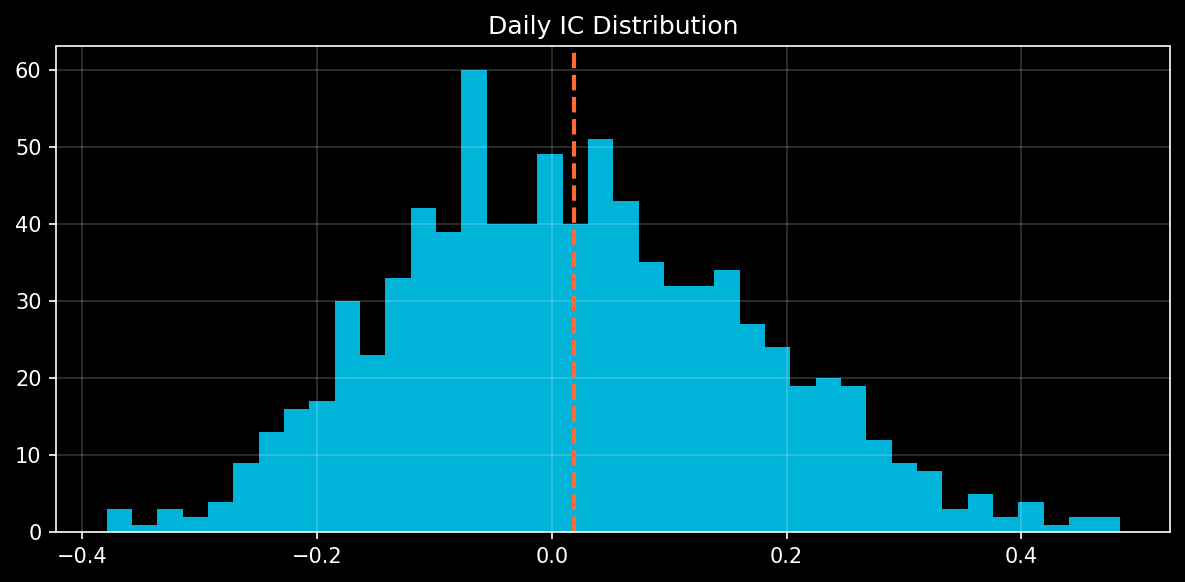
\includegraphics[width=0.88\columnwidth]{significance_ic_distribution.png}
\caption{Distribution of daily IC values. The mean is positive but daily dispersion is large, which explains the modest statistical strength.}
\label{fig:ic_dist}
\end{figure}

Robustness analysis gives three practical conclusions. First, direct use of the ranking head is the strongest fixed execution signal in the saved predictions. Second, $k=10$ is the best top-$k$ setting in the fixed-score sweep. Third, the configured strategy remains profitable under cost stress, declining from 71.71\% annualized return at 0 bps to 45.18\% at 20 bps. The main weakness is persistent drawdown: both the configured and rank-head portfolios experience maximum drawdown around 65\%.

\begin{table}[!t]
\centering
\caption{Selected robustness slices from the configured saved run. Cost sensitivity uses top-$10$ weekly long--short portfolios with the configured score. Rebalance sensitivity changes only the rebalance frequency. Yearly rows use the configured score within each calendar year.}
\label{tab:robustness}
\scriptsize
\setlength{\tabcolsep}{3pt}
\begin{tabular}{llrrrr}
\toprule
Section & Setting & Ann. Ret. & Sharpe & Max DD & Turn. \\
\midrule
Cost & 0 bps & 71.71\% & 1.73 & -62.33\% & 83.98 \\
Cost & 10 bps & 57.90\% & 1.49 & -64.98\% & 83.98 \\
Cost & 20 bps & 45.18\% & 1.24 & -67.49\% & 83.98 \\
\midrule
Rebalance & Daily & 65.56\% & 1.65 & -68.44\% & 123.33 \\
Rebalance & Weekly & 57.90\% & 1.49 & -64.98\% & 83.98 \\
Rebalance & Monthly & -4.30\% & 0.06 & -80.32\% & 37.50 \\
\midrule
Year & 2021 & 89.91\% & 2.07 & -39.28\% & 69.98 \\
Year & 2022 & 26.92\% & 0.80 & -50.41\% & 88.71 \\
Year & 2023 & 8.12\% & 0.41 & -45.76\% & 78.08 \\
Year & 2024 & 212.98\% & 3.54 & -29.59\% & 93.57 \\
\bottomrule
\end{tabular}
\end{table}

\begin{figure}[H]
\centering
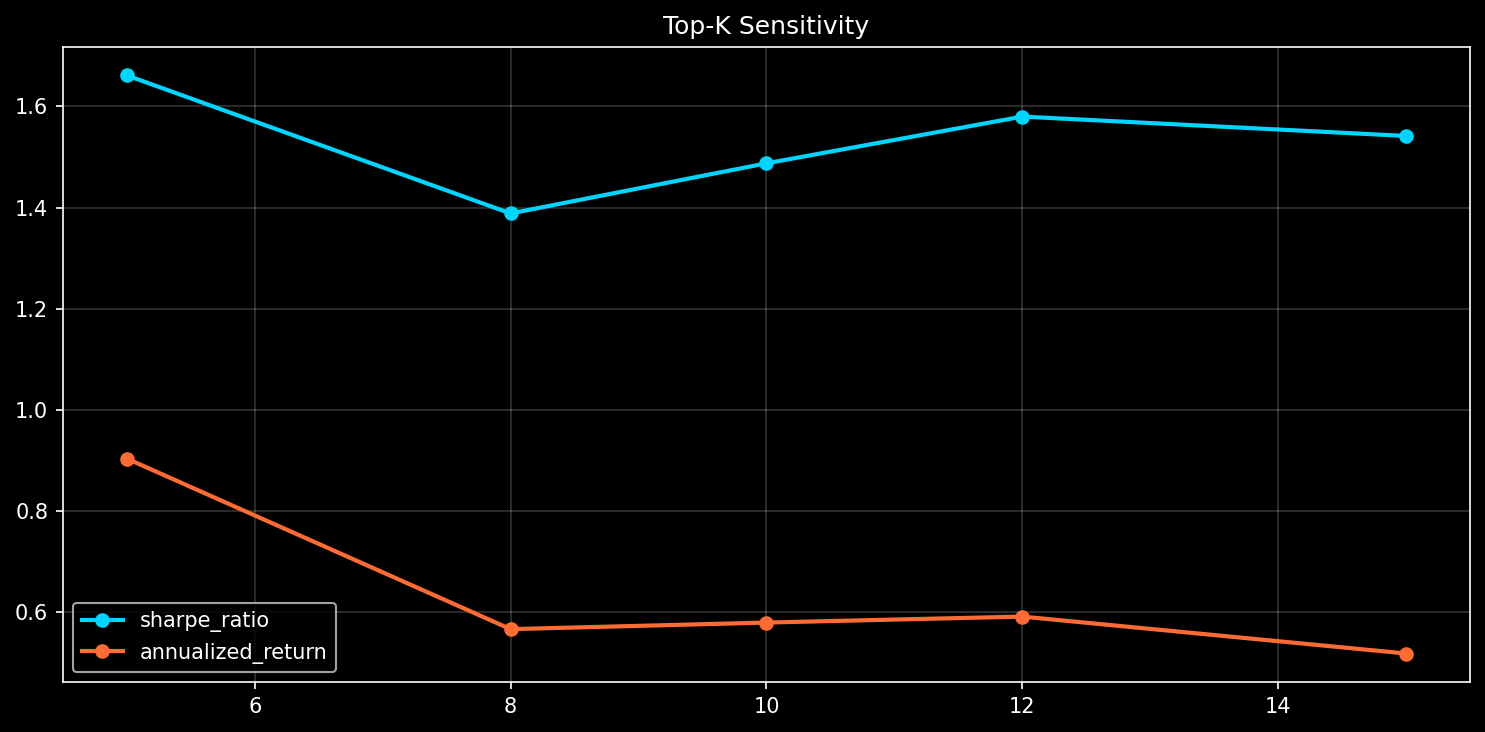
\includegraphics[width=0.88\columnwidth]{robustness_topk.png}
\caption{Top-$k$ robustness sweep. The ranking-head portfolio peaks at $k=10$, while wider portfolios reduce concentration only partially.}
\label{fig:topk}
\end{figure}

Overall, the results support a balanced conclusion. The proposed architecture extracts positive cross-sectional information and its components are empirically meaningful, but it is not unambiguously superior to every simpler baseline under the configured execution score. The strongest claim supported by the evidence is that PatchTST-plus-graph modeling is a useful and extensible research framework for Indian large-cap stock ranking. The evidence does not yet support a production-deployment claim because drawdown and turnover remain too high.

\section{Conclusion}
This paper presented a portfolio-aligned PatchTST-plus-graph framework for NIFTY 100 cross-sectional return forecasting. The system uses 128-day engineered feature histories, multi-scale temporal patch encoding, sector/correlation/embedding-similarity graph attention, market-regime conditioning, and multi-task supervision for return regression, ranking, and direction classification. In walk-forward testing from 2015 to 2024, the configured saved run achieved positive IC, positive Rank IC, 57.90\% annualized return, and a Sharpe ratio of 1.49 after transaction costs. A ranking-head robustness configuration achieved higher return and Sharpe on the same predictions. Baselines and ablations show both strengths and limitations: pretraining, regime features, and graph reasoning matter, but a tabular MLP remains a strong competitor. The final interpretation is therefore deliberately conservative: the project demonstrates a promising research architecture for cross-sectional stock selection, not a deployment-ready trading system.

\section{Future Work}
Future work should focus on four directions. First, stronger sequence baselines such as LSTM, GRU, temporal convolution, transformer-only, and PatchTST-only variants should be added to make the architectural comparison more complete. Second, portfolio construction should include explicit risk controls such as volatility targeting, beta neutrality, sector neutrality, position caps, drawdown-aware exposure scaling, and turnover regularization. Third, the execution layer should be redesigned so that score blending is selected only within validation data and then frozen before test evaluation. Fourth, the data layer should use point-in-time index membership, corporate-action checks, and alternative data vendors to reduce survivorship and data-source bias.

\section*{Acknowledgement}
The authors gratefully acknowledge PES University and the Department of Computer Science and Engineering for their academic support and guidance during this work. The authors also acknowledge the open-source Python ecosystem used in this work, including PyTorch, PyTorch Geometric, pandas, NumPy, scikit-learn, yfinance, and Matplotlib. The authors further acknowledge that the present repository is a research prototype and that any investment use would require independent validation, risk controls, and compliance review.

\bibliographystyle{IEEEtran}
\bibliography{references}

\end{document}
